\chapter{Persistence Length Appendix}
\label{app:pers_len}

\begin{table}[ht]
    \centering
    \begin{tabular}{ll}

    \textbf{Polymer}  &     \textbf{Density} \\
    \hline
    PCPDTFBT-C1-BO    &     0.05    \\
    PCPDTFBT-C3-BO    &     0.05    \\
    PCPDTFBT-C4-BO    &     0.01    \\
    PCPDTFBT-C5-BO    &     0.05    \\
    PCPDTFBT-C11-BO   &     0.005   \\ 
    PCPDTPT-ene-HD    &     0.005   \\
    PCPDTPT-ene-ODD   &     0.05    \\
    PCPDTPT-HD        &     0.05    \\
    PCPDTPT-nC16      &     0.05    \\
    PCPDTPT-ODD       &     0.05    \\
    PIDTBT-nC16       &     0.05    \\
    PIDTCPDT-C11-BO   &     0.05    \\
    PIDTFBT-C11-BO    &     0.005   \\
    \end{tabular}
    \caption{Densities at which each polymer simulation was run at. All densities reported in units of g/mL}
    \label{densities}
\end{table}

\begin{table}[ht]
    \centering
    \begin{tabular}{l|l}
        \textbf{Polymer} & \textbf{TPS} \\
        \hline
        \textbf{PCPDTFBT-C11-BO  }   &       1027.1953   \\
        \textbf{PCPDTFBT-C1-BO   }    &       1085.1254   \\
        \textbf{PCPDTFBT-C3-BO   }   &       1134.8646   \\
        \textbf{PCPDTFBT-C4-BO   }   &       1021.8457   \\
        \textbf{PCPDTFBT-C5-BO   }   &       959.0328    \\
        \textbf{PCPDTPT-ene-HD   }    &       1987.0726   \\
        \textbf{PCPDTPT-ene-ODD  }    &       1717.0476   \\
        \textbf{PCPDTPT-HD       }   &       1443.4256   \\
        \textbf{PCPDTPT-nC16     }   &       1481.9449   \\
        \textbf{PCPDTPT-ODD      }   &       1425.6319   \\
        \textbf{PIDTBT-nC16      }   &       1025.8267   \\
        \textbf{PIDTCPDT-C11-BO  }   &       646.3932    \\
        \textbf{PIDTFBT-C11-BO   }   &       421.9683    \\
    \end{tabular}
    \caption{Average timesteps per second (TPS) for each polymer simulation. Values averaged over each simulation with temperatures ranging from 252 K to 2013 K.}
    \label{tab:pl_tps}
\end{table}

\begin{table}[ht]
    \centering
    \begin{tabular}{c|c|c|c|c}
                        &  \multicolumn{4}{c}{\textbf{l\textsubscript{p}}}  \\
        \hline
        \textbf{Polymer}  & \textbf{252 K} & \textbf{503 K} & \textbf{1006 K} & \textbf{SANS}\\
        \hline
        PCPDTFBT-C1-BO    &   $37.8 \pm 0.1$    &	$115.3 \pm 0.5$   &   $99.7 \pm 5.9$     &    67	 \\
        PCPDTFBT-C3-BO    &   $47.5 \pm 0.1$    &	$57.6 \pm 0.8$    &   $98.9 \pm 6.1$     &    78.4   \\
        PCPDTFBT-C4-BO    &   $46.3 \pm 0.3$    &	$65.8 \pm 0.9$    &   $105.1 \pm 5.6$    &    86.4   \\
        PCPDTFBT-C5-BO    &   $35.4 \pm 0.1$    &	$68.7\pm 0.5$     &   $104.3 \pm 7.8$    &    114	 \\
        PCPDTFBT-C11-BO   &   $34.6 \pm 0.1$    &	$55.9 \pm 0.7$    &   $104.0 \pm 7.4$    &    291	 \\
        PCPDTPT-ene-HD    &   $39.8 \pm 0.4$    &	$48.4 \pm 0.3$    &   $110.7 \pm 7.9$    &    76.6   \\
        PCPDTPT-ene-ODD   &   $21.9 \pm 0.1$    &	$38.5 \pm 0.3$    &   $97.8 \pm 7.3$     &    83.4   \\
        PCPDTPT-HD        &   $36.8 \pm 0.1$    &	$55.3 \pm 2.6$    &   $100.4 \pm 6.3$    &    47.3   \\
        PCPDTPT-nC16      &   $40.2 \pm 0.2$    &	$60.3 \pm 0.4$    &   $96.0 \pm 6.3$     &    61     \\
        PCPDTPT-ODD       &   $56.4 \pm 0.3$    &	$63.6 \pm 0.7$    &   $99.6 \pm 9.6$     &    54.9   \\
        PIDTBT-nC16       &   $65.4\pm 0.2$     &	$57.8 \pm 0.4$    &   $200.6 \pm 25.5$   &    1310   \\
        PIDTCPDT-C11-BO   &   $36.0 \pm 0.1$    &	$76.4 \pm 2.4$    &   $182.2 \pm 13.7$   &    236	 \\
        PIDTFBT-C11-BO    &   $79.4 \pm 1.1$    &	$90.6 \pm 6.5$    &   $178.4 \pm 9.2$    &    254	 \\
    \end{tabular}
    \caption{Caption}
    \label{tab:l_p}
\end{table}

\begin{table}[ht]
    \centering
    \begin{tabular}{c|c}
    \textbf{Polymer}   &    \textbf{$T_{SANS}$}\\
    \hline
    PCPDTFBT-C1-BO     &    326\\
    PCPDTFBT-C3-BO     &    736\\
    PCPDTFBT-C4-BO     &    767\\
    PCPDTFBT-C5-BO     &    1091\\
    PCPDTFBT-C11-BO    &    3035\\
    PCPDTPT-ene-HD     &    692\\
    PCPDTPT-ene-ODD    &    885\\
    PCPDTPT-HD         &    389\\
    PCPDTPT-nC16       &    526\\
    PCPDTPT-ODD        &    278\\
    PIDTBT-nC16        &    6785\\
    PIDTCPDT-C11-BO    &    1290\\
    PIDTFBT-C11-BO     &    1591\\
    \end{tabular}
    \caption{Predicted simulation temperature at which $l_p^{MD}$ would match $l_p^{SANS}$.}
    \label{tab:T_sans}
\end{table}

\newpage % NOTE: The appendix title should be on its own page.

\begin{figure}
    \centering
    \includegraphics[width=1\linewidth]{src/figures/pers_l_figs/pers_len1.png}
    \label{fig:pers_len1}
\end{figure}

\newpage 

\begin{figure}
    \centering
    \includegraphics[width=1\linewidth]{src/figures/pers_l_figs/pers_len2.png}
    \label{fig:pers_len2}
\end{figure}

\newpage 

\begin{figure}
    \centering
    \includegraphics[width=1\linewidth]{src/figures/pers_l_figs/pers_len3.png}
    \label{fig:pers_len3}
\end{figure}

\clearpage

\begin{figure}
    \centering
    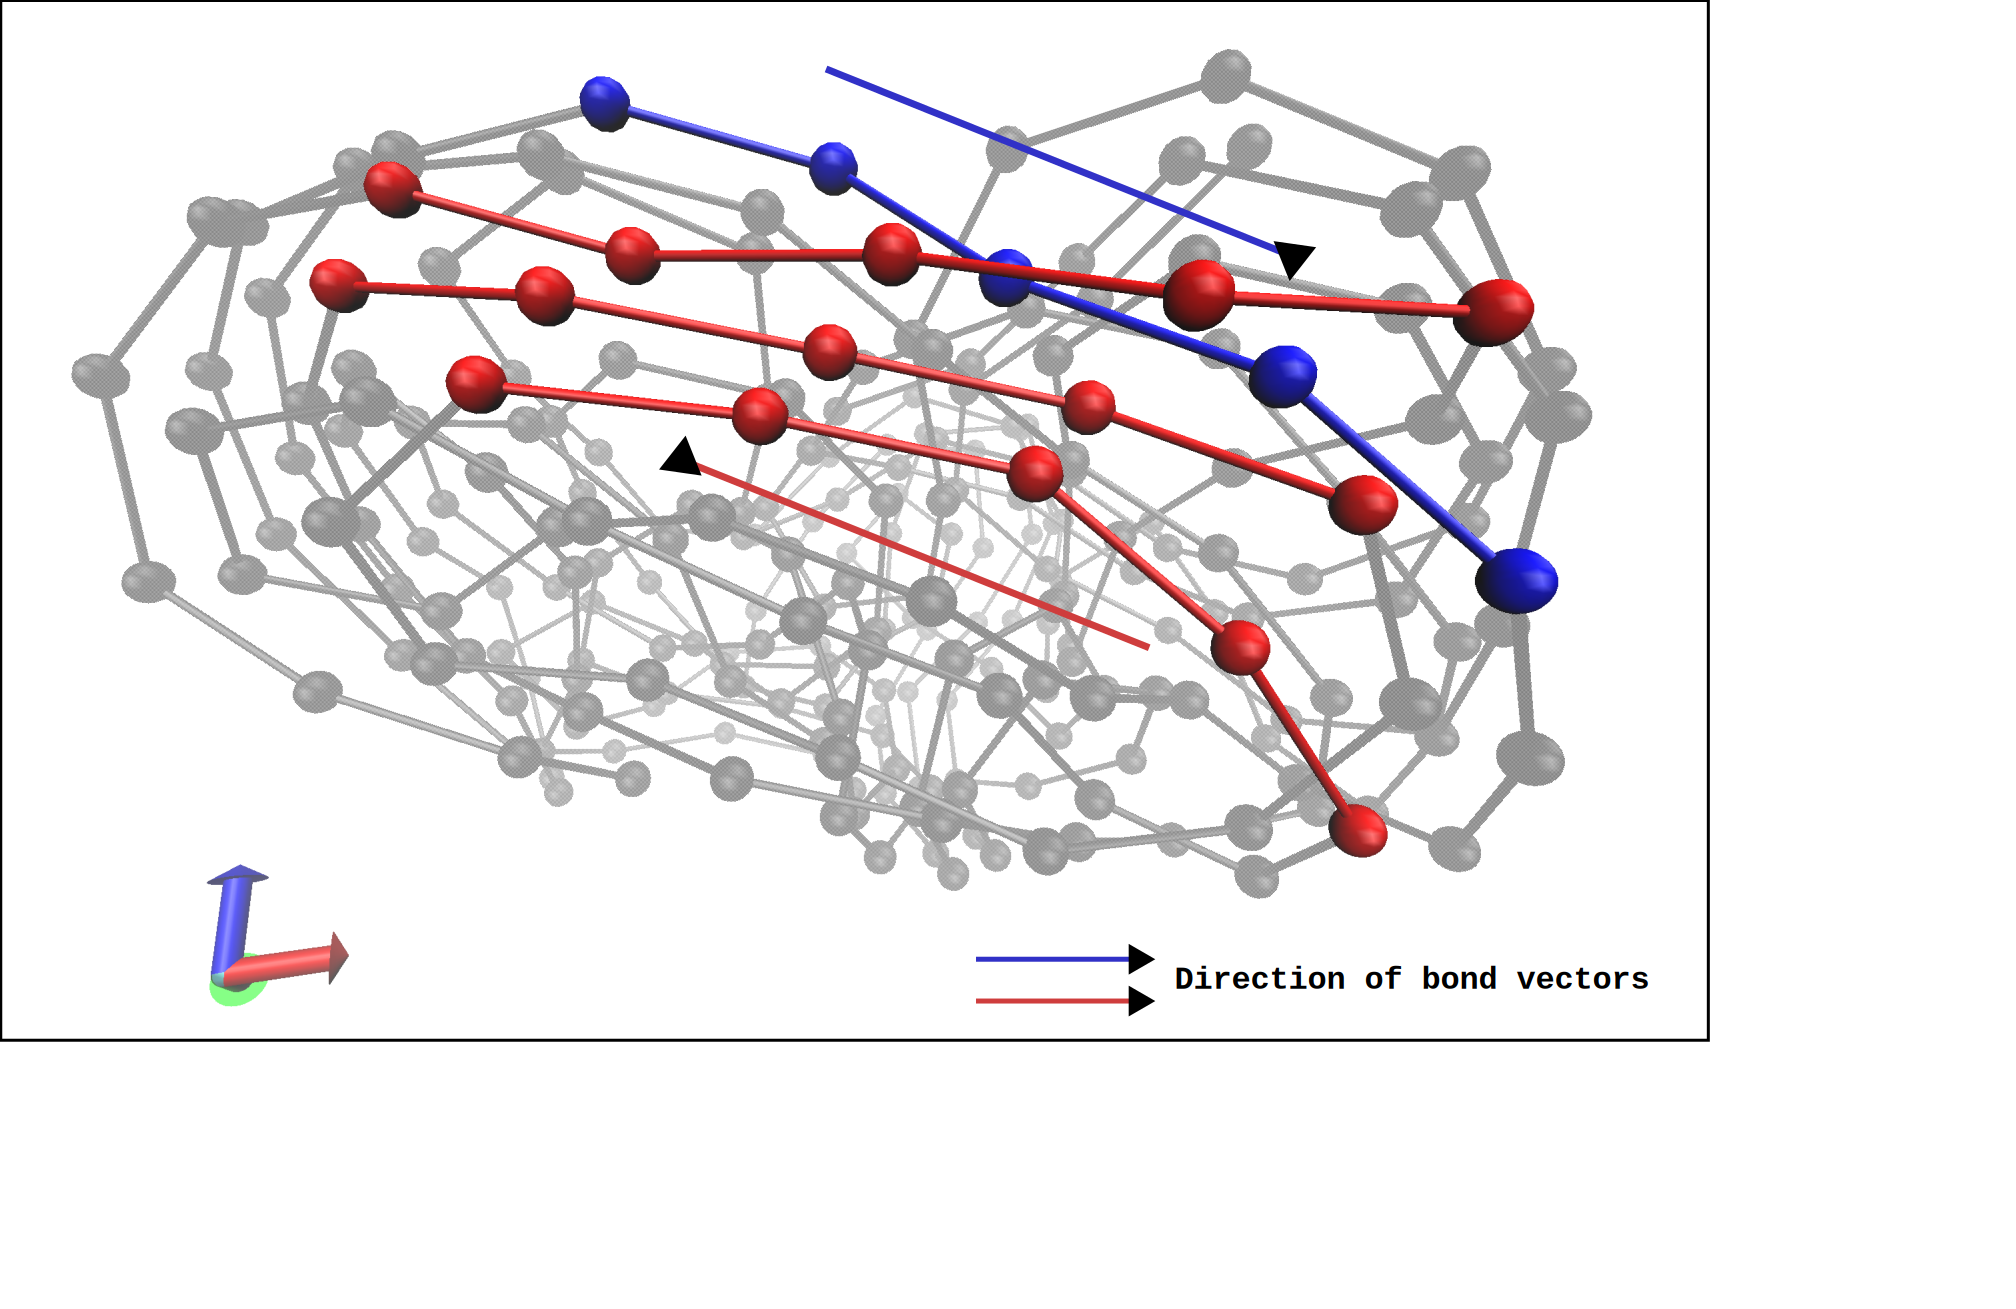
\includegraphics[width=1\linewidth]{src/figures/pers_l_figs/real_cond_polymer.png}
    \caption{Snapshot of coarse grained PCPDTPT-HD at a temperature of 252 K and density of 0.05 g/mol. The red highlighted CG beads have parallel aligned bond vectors. The blue highlighted CG beads are parallel, but anti-aligned with the red.}
    \label{fig:real_cond_polymer}
\end{figure}


\begin{figure}
    \centering
    \includegraphics[width=1\linewidth]{src/figures/pers_l_figs/untitled folder/pcpdtpt/eneHD_plot.jpeg}
    \caption{Persistence length ($l_p^{MD}$) of PCPDTPT-eneHD vs Temperature plot with a linear regression calculated using SciPy \citep{2020SciPy-NMeth} and $T_{SANS}$ prediction.}
    \label{fig:eneHD_plot}
\end{figure}

\begin{figure}
    \centering
    \includegraphics[width=1\linewidth]{src/figures/pers_l_figs/untitled folder/pcpdtpt/eneODD_plot.jpeg}
    \caption{Persistence length ($l_p^{MD}$) of PCPDTPT-eneODD vs Temperature plot with a linear regression calculated using SciPy \citep{2020SciPy-NMeth} and $T_{SANS}$ prediction.}
    \label{fig:eneODD_plot}
\end{figure}

\begin{figure}
    \centering
    \includegraphics[width=1\linewidth]{src/figures/pers_l_figs/untitled folder/pcpdtpt/HD_plot.jpeg}
    \caption{Persistence length ($l_p^{MD}$) of PCPDTPT-HD vs Temperature plot with a linear regression calculated using SciPy \citep{2020SciPy-NMeth} and $T_{SANS}$ prediction.}
    \label{fig:HD_plot}
\end{figure}

\begin{figure}
    \centering
    \includegraphics[width=1\linewidth]{src/figures/pers_l_figs/untitled folder/pcpdtpt/ODD_plot.jpeg}
    \caption{Persistence length ($l_p^{MD}$) of PCPDTPT-ODD vs Temperature plot with a linear regression calculated using SciPy \citep{2020SciPy-NMeth} and $T_{SANS}$ prediction.}
    \label{fig:ODD_plot}
\end{figure}

\begin{figure}
    \centering
    \includegraphics[width=1\linewidth]{src/figures/pers_l_figs/untitled folder/pcpdtpt/nC16_plot.jpeg}
    \caption{Persistence length ($l_p^{MD}$) of PCPDTPT-nC16 vs Temperature plot with a linear regression calculated using SciPy \citep{2020SciPy-NMeth} and $T_{SANS}$ prediction.}
    \label{fig:nC16_plot}
\end{figure}


\begin{figure}
    \centering
    \includegraphics[width=1\linewidth]{src/figures/pers_l_figs/untitled folder/pcpdtfbt/C1_plot.jpeg}
    \caption{Persistence length ($l_p^{MD}$) of PCPDTFBT-C1-BO vs Temperature plot with a linear regression calculated using SciPy \citep{2020SciPy-NMeth} and $T_{SANS}$ prediction.}
    \label{fig:C1_plot}
\end{figure}

\begin{figure}
    \centering
    \includegraphics[width=1\linewidth]{src/figures/pers_l_figs/untitled folder/pcpdtfbt/C3_plot.jpeg}
    \caption{Persistence length ($l_p^{MD}$) of PCPDTFBT-C3-BO vs Temperature plot with a linear regression calculated using SciPy \citep{2020SciPy-NMeth} and $T_{SANS}$ prediction.}
    \label{fig:C3_plot}
\end{figure}

\begin{figure}
    \centering
    \includegraphics[width=1\linewidth]{src/figures/pers_l_figs/untitled folder/pcpdtfbt/c4_plot.jpeg}
    \caption{Persistence length ($l_p^{MD}$) of PCPDTFBT-C4-BO vs Temperature plot with a linear regression calculated using SciPy \citep{2020SciPy-NMeth} and $T_{SANS}$ prediction.}
    \label{fig:C4_plot}
\end{figure}

\begin{figure}
    \centering
    \includegraphics[width=1\linewidth]{src/figures/pers_l_figs/untitled folder/pcpdtfbt/C5_plot.jpeg}
    \caption{Persistence length ($l_p^{MD}$) of PCPDTFBT-C5-BO vs Temperature plot with a linear regression calculated using SciPy \citep{2020SciPy-NMeth} and $T_{SANS}$ prediction.}
    \label{fig:C5_plot}
\end{figure}

\begin{figure}
    \centering
    \includegraphics[width=1\linewidth]{src/figures/pers_l_figs/untitled folder/pcpdtfbt/C11_plot.jpeg}
    \caption{Persistence length ($l_p^{MD}$) of PCPDTFBT-C11-BO vs Temperature plot with a linear regression calculated using SciPy \citep{2020SciPy-NMeth} and $T_{SANS}$ prediction.}
    \label{fig:C11_plot}
\end{figure}


\begin{figure}
    \centering
    \includegraphics[width=1\linewidth]{src/figures/pers_l_figs/untitled folder/idt/nc16_plot.jpeg}
    \caption{Persistence length ($l_p^{MD}$) of PIDTBT-nC16 vs Temperature plot with a linear regression calculated using SciPy \citep{2020SciPy-NMeth} and $T_{SANS}$ prediction.}
    \label{fig:idtnc16_plot}
\end{figure}

\begin{figure}
    \centering
    \includegraphics[width=1\linewidth]{src/figures/pers_l_figs/untitled folder/idt/cpdt_plot.jpeg}
    \caption{Persistence length ($l_p^{MD}$) of PIDTCPDT-C11-BO vs Temperature plot with a linear regression calculated using SciPy \citep{2020SciPy-NMeth} and $T_{SANS}$ prediction.}
    \label{fig:idtcpdt_plot}
\end{figure}

\begin{figure}
    \centering
    \includegraphics[width=1\linewidth]{src/figures/pers_l_figs/untitled folder/idt/fbt_plot.jpeg}
    \caption{Persistence length ($l_p^{MD}$) of PIDTFBT-C11-BO vs Temperature plot with a linear regression calculated using SciPy \citep{2020SciPy-NMeth} and $T_{SANS}$ prediction.}
    \label{fig:idt_fbt_plot}
\end{figure}


\begin{figure}
    \centering
    \includegraphics[width=0.6\linewidth]{src/figures/pers_l_figs/e-e plots/C1.png}
    \caption{$\sqrt{\langle R^2 \rangle}$ vs Temperature for PCPDTFBT-C1-BO with a linear regression for the linear portion of the plot. Horizontal line plotted at $\sqrt{N_b}*l_b$.}
    \label{fig:e-e_C1}
\end{figure}

\begin{figure}
    \centering
    \includegraphics[width=0.6\linewidth]{src/figures/pers_l_figs/e-e plots/C3.png}
    \caption{$\sqrt{\langle R^2 \rangle}$ vs Temperature for PCPDTFBT-C3-BO with a linear regression for the linear portion of the plot. Horizontal line plotted at $\sqrt{N_b}*l_b$.}
    \label{fig:e-e_C3}
\end{figure}

\begin{figure}
    \centering
    \includegraphics[width=0.6\linewidth]{src/figures/pers_l_figs/e-e plots/C4.png}
    \caption{$\sqrt{\langle R^2 \rangle}$ vs Temperature for PCPDTFBT-C4-BO with a linear regression for the linear portion of the plot. Horizontal line plotted at $\sqrt{N_b}*l_b$.}
    \label{fig:e-e_C4}
\end{figure}

\begin{figure}
    \centering
    \includegraphics[width=0.6\linewidth]{src/figures/pers_l_figs/e-e plots/C5.png}
    \caption{$\sqrt{\langle R^2 \rangle}$ vs Temperature for PCPDTFBT-C5-BO with a linear regression for the linear portion of the plot. Horizontal line plotted at $\sqrt{N_b}*l_b$.}
    \label{fig:e-e_C5}
\end{figure}

\begin{figure}
    \centering
    \includegraphics[width=0.6\linewidth]{src/figures/pers_l_figs/e-e plots/C11.png}
    \caption{$\sqrt{\langle R^2 \rangle}$ vs Temperature for PCPDTFBT-C11-BO with a linear regression for the linear portion of the plot. Horizontal line plotted at $\sqrt{N_b}*l_b$.}
    \label{fig:e-e_C11}
\end{figure}

\begin{figure}
    \centering
    \includegraphics[width=0.6\linewidth]{src/figures/pers_l_figs/e-e plots/ene_HD.png}
    \caption{$\sqrt{\langle R^2 \rangle}$ vs Temperature for PCPDTPT-ene-HD with a linear regression for the linear portion of the plot. Horizontal line plotted at $\sqrt{N_b}*l_b$.}
    \label{fig:e-e_ene_HD}
\end{figure}

\begin{figure}
    \centering
    \includegraphics[width=0.6\linewidth]{src/figures/pers_l_figs/e-e plots/ene_ODD.png}
    \caption{$\sqrt{\langle R^2 \rangle}$ vs Temperature for PCPDTPT-ene-ODD with a linear regression for the linear portion of the plot. Horizontal line plotted at $\sqrt{N_b}*l_b$.}
    \label{fig:e-e_ene_ODD}
\end{figure}

\begin{figure}
    \centering
    \includegraphics[width=0.6\linewidth]{src/figures/pers_l_figs/e-e plots/HD.png}
    \caption{$\sqrt{\langle R^2 \rangle}$ vs Temperature for PCPDTPT-HD with a linear regression for the linear portion of the plot. Horizontal line plotted at $\sqrt{N_b}*l_b$.}
    \label{fig:e-e_HD}
\end{figure}

\begin{figure}
    \centering
    \includegraphics[width=0.6\linewidth]{src/figures/pers_l_figs/e-e plots/nC16.png}
    \caption{$\sqrt{\langle R^2 \rangle}$ vs Temperature for PCPDTPT-nC16 with a linear regression for the linear portion of the plot. Horizontal line plotted at $\sqrt{N_b}*l_b$.}
    \label{fig:e-e_nC16}
\end{figure}

\begin{figure}
    \centering
    \includegraphics[width=0.6\linewidth]{src/figures/pers_l_figs/e-e plots/ODD.png}
    \caption{$\sqrt{\langle R^2 \rangle}$ vs Temperature for PCPDTPT-ODD with a linear regression for the linear portion of the plot. Horizontal line plotted at $\sqrt{N_b}*l_b$.}
    \label{fig:e-e_ODD}
\end{figure}

\begin{figure}
    \centering
    \includegraphics[width=0.6\linewidth]{src/figures/pers_l_figs/e-e plots/PIDT_nC16.png}
    \caption{$\sqrt{\langle R^2 \rangle}$ vs Temperature for PIDTBT-nC16 with a linear regression for the linear portion of the plot. Horizontal line plotted at $\sqrt{N_b}*l_b$.}
    \label{fig:e-e_PIDTBT}
\end{figure}

\begin{figure}
    \centering
    \includegraphics[width=0.6\linewidth]{src/figures/pers_l_figs/e-e plots/PIDT_CPDT.png}
    \caption{$\sqrt{\langle R^2 \rangle}$ vs Temperature for PIDTCPDT-C11-BO with a linear regression for the linear portion of the plot. Horizontal line plotted at $\sqrt{N_b}*l_b$.}
    \label{fig:e-e_PIDTCPDT}
\end{figure}

\begin{figure}
    \centering
    \includegraphics[width=0.6\linewidth]{src/figures/pers_l_figs/e-e plots/PIDT_FBT.png}
    \caption{$\sqrt{\langle R^2 \rangle}$ vs Temperature for PIDTBFT-C11-BO with a linear regression for the linear portion of the plot. Horizontal line plotted at $\sqrt{N_b}*l_b$.}
    \label{fig:e-e_FBT}
\end{figure}